\Chapter{Koncepció}
% TODO: Le kellene írni az OBJ formátumról a fontosabb dolgokat!
\Section{OBJ fájlformátum}

Az OBJ fájlformátumot elsőnek a Wavefront Technologies kezdte kifejleszteni az 1980-as években az Advanced Visualizer animációs csomagjához. Ez a formátum egy olyan karakteres fájlformátum, ami utat enged geometriai objektumok leírásának egy aránylag egyszerű és egységes formában \cite{martinreddy}.

Magát a formátumot ott logikus használni, ahol egyszerű modelleket jelenítünk meg és ezeket nem akarjuk animálni. Például egy olyan egyszerű autó szimulátoros játéknál, ahol maga az autó geometriáját tekintve nem változik maximum a pozíciója és az orientációja, ezeket a transzformációs mátrix állításával egyszerűen megadhatjuk, így nincs szükség a modell animálására.

\SubSection{Wavefront obj fájlformátum}

A formátum általános felépítése a kevetkezőképpen alakul.
Minden sor áll egy kezdő karakterből vagy szimbólumból, utána egy elválasztójel (szóköz vagy tabulátor). Rögtön ezután szám vagy szöveg következik.

Minden karakter, ami egy kettőskereszt (\#) karakter után helyezkedik el, az egy megjegyzés, például
\begin{python}
# ez egy megjegyzes
\end{python}
A \textbf{v} kezdőbetűvel ellátott sorok \textsl{geometriai csúcsot} definiálnak. Ezt követik a koordináták $(x, y, z [, w])$. (A szögletes zárójel opcionális koordinátát jelent ebben az esetben, amelynek alapértelmezett értéke 1.) Egy csúcspontot leíró sor például a következőképpen néz ki:
\begin{python}
v -0.123 0.345 0.678
\end{python}
A \textbf{vt} kezdőbetűvel \textsl{textúra koordinátát} írunk le. Ezt (u, [, v, w]) koordináták követik, ezek 0 és 1 közötti értékek. A szögletes zárójel [ ] koordináta értékei opcionálisak és alapértelmezés szerint 0.0 az értékük.
\begin{python}
vt 0.500 1 [0]
\end{python}
\bigskip
A \textbf{vn} kezdőbetűs sorok \textsl{normál vektorokat} definiálnak. Ezt $(x, y, z)$ koordináták követik.
\begin{python}
vn -0.500 0.500 -0.500
\end{python}
\bigskip
Az \textbf{f} kezdőbetűvel egy \textsl{lap elemet} írunk le. A \textsl{lap elemet} \textsl{geometriai csúcs}, \textsl{textúra koordináta}, \textsl{normál csúcs} indexek listájával adjuk meg, {/} jellel elválasztva. Csúcs{\_}index {/} textura{\_}index {/}  normál{\_}index formátumban. Minden index 1-ről indul és növekszik annak sorrendjében, amelyben a hivatkozott elemet definiálták.\\

\SubSection{Lap definiálási formák}

A kizárólagosan \textsl{geometriai csúcsokból} álló lapot a következő formában definiálja a szabvány:
\begin{python}
f v1 v2 v3 v4 ...
\end{python}
Amennyiben minden \textsl{geometriai csúcshoz} hozzá van rendelve egy \textsl{textúra koordináta} is, akkor az az alábbi forma szerint néz ki:
\begin{python}
f v1/vt1 v2/vt2 v3/vt3 ...
\end{python}
\bigskip
Minden \textsl{geometriai csúcs} tartalmazhat \textsl{textúra koordinátát} és \textsl{normál csúcsot} az alábbiak szerint:
\begin{python}
f v1/vt1/vn1 v2/vt2/vn2 v3/vt3/vn3 ...
\end{python}
Előfordulhat, hogy a \textsl{geometriai csúcshoz} csak a \textsl{normál csúcs} lett hozzárendelve, vagyis a \textsl{textúra koordináta} opcionális:
\begin{python}
f v1/ /vn1 v2/ /vn2 v3/ /vn3 ...
\end{python}

Összefoglalva, az OBJ formális nyelv kulcsszavakból (<\textbf{v}>, <\textbf{vt}>, <\textbf{vn}>, <\textbf{f}>), speciális karakterekből (<\textbf{/}>,<\textbf{\#}>) és számokból (<\textbf{Float}>, <\textbf{Integer}>) épül fel. Az OBJ nyelvtanát a következő szabályokkal adhatjuk meg:

\bigskip

\noindent(OBJFájl) = {(Geometriai csúcs)}+{(Textúra koordináta)}+{(Normál csúcs)}+{(Lapelem)}\\
(Geometriai csúcs) = (v)+(Float)+(Float)+(Float)\\
(Textúra koordináta) = (vt)+(Float)+(Float)+[0]\\
(Normál csúcs) = (vn)+(Float)+(Float)+(Float)\\
(Lapelem) = (f)+{(Lap{\_}indexek)}\\
(Lap{\_}indexek) = (Integer)+[(/)+[(Integer)]+[(/)+[(Integer)]]]\\

\noindent A szögeltes zárójelbe foglalt elemek opcionálisak, vagyis a bennük lévő fogalom egyszer vagy egyszer sem jelenik meg a leírás során.

A következőkben egy példát láthatunk arra, hogy egy négyszög hogyan definiálható a Wavefront szabvány segítségével.
\begin{python}
v 0.0 0.0 0.0
v 1.0 0.0 0.0
v 1.0 1.0 0.0
v 0.0 1.0 0.0

vt 0.0 0.0
vt 1.0 0.0
vt 1.0 1.0
vt 0.0 1.0

vn 1.0 0.0 0.0

f 1/1/1 2/2/1 3/3/1 4/4/1
\end{python}
A fájl először felsorolja a \textsl{geometriai csúcsokat} (\textbf{v}), utána a \textsl{textúra koordinátákat} (\textbf{vt}) és \textsl{normál csúcsokat} (\textbf{vn}), majd az \textsl{lap elemekkel} (\textbf{f}) egymáshoz rendeli ezeket. Ebben az esetben például a lapot négy csúcsponttal adtuk meg és {/} jellel elválasztva hozzá rendeltük a  \textsl{geometriai csúcsok}, a \textsl{textúra koordináták} és a \textsl{normál csúcsok} sorszámát.

A teljes OBJ formátum nagyon összetett, sok olyan szerkezeti egységet tartalmaz, ami egy szimpla objektum modellezéséhez általában nem szükséges.

\Section{Anyagjellemzők leírása}

Az OBJ formátum 3D térben lévő objektumok csupán geometriáját írja le. Ezért szükségünk van még az anyagjellemzőkre is a képszintézis során. A különböző anyagokat fizikai jellemzőikkel írjuk le. Ezek a jellemzők például fényáteresztő képesség, fényvisszaverő képesség, törésmutató \cite{diane1995mtl}.

\SubSection{Az MTL fájl felépítése}

Ezeket a tulajdonságokat az MTL (\textit{Material Template Library}) tartalmazza, a formátum hasonlóan az OBJ formátumhoz szintén szöveges. Az OBJ fájl tartalmazza a hivatkozást az {MTL} fájlra: \cite{diane1995mtl}.
\begin{python}
mtllib fajlnev.mtl
\end{python}
Az \texttt{mtllib} hivatkozza be az MTL fájlt, ezután a \textsl{fájlnév} és a kiterjesztés következik (ez esetben \texttt{.mtl}).

OBJ fájlból akár egynél több anyagfájlra is lehet hivatkozni és egy MTL fájl tartalmazhat akár több anyagdefiníciót is.

A következő hívatkozással lehet beállítani a következő anyag anyagdefinícióját:
\begin{python}
usemtl (anyag neve)
\end{python}
Az anyag neve azonos egy anyagmeghatározással egy külső MTL fájlban.

Az objektumokat és sokszögcsoportokat a következő hivatkozások adják meg.
\begin{python}
o [objektum neve]
  ...
  g [csoport neve]
  ...
\end{python}

Sokszögek közötti árnyékolás a következővel állítható:
\begin{python}
s 1
  ...
  s ki
  ...
\end{python}

\SubSection{Több anyagjellemző megadása}

Az MTL fájl az anyagokat egymás után definiálja a fájlban, ahol az egyes leírások a \texttt{newmtl} paranccsal kezdődnek, például
\begin{python}
newmtl szines
\end{python}
A \texttt{newmtl} egy új anyagot definiál, aminek a neve \texttt{"szines"}.

A \textbf{Ka} kulcsszó az anyag ambiens, környezettől független színét adja. Ez úgy viselkedik, mintha az anyag világítana, szóval ha a testet nem éri fény abban az esetben is ilyen lesz a színe. Viszont  az ambient tulajdonság nem viselkedik fényforrásként, attól hogy egy testnek ambiens színe van, az nem fogja megvilágítani a körülötte lévő többi testet. Az értéke vörös, zöld és kék színösszetevőkkel (RGB-vel) van megadva 0 és 1 között.
\begin{python}
Ka 1.000 1.000 1.000
\end{python}

A \textbf{Kd} kulcsszó az anyag diffúz színét határozza meg. Ez a tulajdonság a test színét írja le, lényegében a diffúz tulajdonság meghatározza, egy felület rá eső fény mely részét nyeli el. Az értéke szintén RGB-vel van megadva 0 és 1 között.
\begin{python}
Kd 1.000 1.000 1.000
\end{python}

A \textbf{Ks} kulcsszó az anyag spekuláris színét adja. Ez az anyag tükröződéséért felelős. Értéke 0 és 1 között állítható. Amennyiben azt szeretnénk hogy az anyag minden ráeső fényt visszaverjen (tükörként működve), abban az esetben $(1, 1, 1)$ értéket kell megadni ha pedig azt, hogy mindet elnyeljen akkor $(0, 0, 0)$ értékeket. Ennek megadására egy példa az alábbi
\begin{python}
Ks 1.000 1.000 1.000
\end{python}

Az \textbf{Ns} kulcsszó az anyag \textit{shininess} évtékét, vagyis csillogását adja. Az anyagok felszíne nem csak tükörszerűen viselkedhetnek, hanem van saját fényük is. Ennek az értéke 0 és 1000 között határozható meg. Ezen skálán minél nagyobb értéket kap, annál nagyobb lesz a fénysávok élessége.\cite{johnmtl}
\begin{python}
Ns 10.000
\end{python}

\Section{Textúrák}

Bár az OBJ formátumnak nem része, mégis fontos megemlíteni a textúrázást. A valósághű képek létrehozásánál egy fontos eszközünk a képként megadott mintázatok térbeli objektumokra való leképzése, hiszen a valóságban körülöttünk lévő tárgyak sem egyszínűek.

Textúrázás alatt általában kétdimenziós textúrázást értünk, de lehetnek ezek akár egy vagy háromdimenziósak is. A textúra geometriailag egy téglalap, ami sorokba és oszlopokba rendezet elemekből épül fel.

A textúra tehát adatok 1, 2 vagy 3 dimenziós tömbjének tekinthető. Az egyes textúra elemekhez tárolt adat képviselhet színt, fényerősséget vagy szín és alfa értékeket, azaz 1, 2, 3 vagy 4 adat  tartozhat minden textúra elemhez.

A téglalap alakú textúrákat azonban tetszőleges alakú sokszögekre, kell ráhelyezni. Ehhez a hozzárendelést a modelltérben kell megadni, ezért  a textúráka is hatnak a modell- és vetítési transzformációk. Ennek érdekében az objektumok létrehozásakor a csúcspontok geometriai koordinátái mellett a textúra koordinátákat is meg kell adni, ezeknek a textúra koordinátáknak $[0, 1] \times [0, 1]$ egységnégyzeten belül kell elhelyezkedniük \cite{juhasz2003opengl}.

\Section{Modellbetöltő szofverek}

Manapság rengeteg modell elemző és betöltő szoftver áll rendelkezésünkre. A legtöbb ilyen szoftverről általánosságban elmondható, hogy ingyenes illetve  nyílt forráskóddal rendelkezik. Akadnak köztük elemzők, online betöltők, illetve telepítés után használható megjelenítők. A következő szakaszokban ezen szoftverek bemutatására kerül sor.

\SubSection{Kixor modell elemző}

Az első vizsgált elemző a Kixor modell elemzőszoftver volt \cite{micah1987markup}.
Ez a következő webcímen érhető el: \url{https://www.kixor.net/dev/objloader/}.

A program elemzi az adott OBJ fájlt, majd kiírja az abban lévő adatok egy részét.

\begin{figure}[h]
\centering
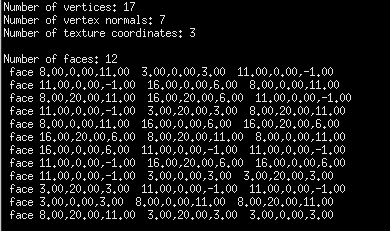
\includegraphics[scale=0.8]{images/kixor.png}
\caption{A \textit{Kixor} elemző szoftver kimenete a \texttt{test.obj} állományra}
\label{fig:kixor}
\end{figure}
\bigskip

\Aref{fig:kixor}. ábrán jól látható módon a program elvégezte a szükséges számításokat majd visszatért a számított adatokkal.

Ez a szoftver nem alkalmas a modell megjelenítésére, csak annak elemzésére viszont azt sok szemppontból megteszi. Amennyiben csak elemezni szeretnénk az OBJ fájlunkat, abban az esetben kiváló lehetőségként szolgál.

\SubSection{Online 3D Viewer}

Az első dolgozatban vizsgált már megjelenítésre is alkalmas szoftver az \textit{Online 3D Viewer} \cite{online2014viktor}.
Ez a \url{https://3dviewer.net/} weboldalon található.

Az oldalra érkezve \aref{fig:model_viewer1}. ábrán látható egyszerű és letisztult felületet kapunk, ahol rövid leírást találhatunk, hogy melyek a támogatott fájlformátumok, illetve azokat hogyan tudjuk megnyitni.

\begin{figure}[h]
\centering
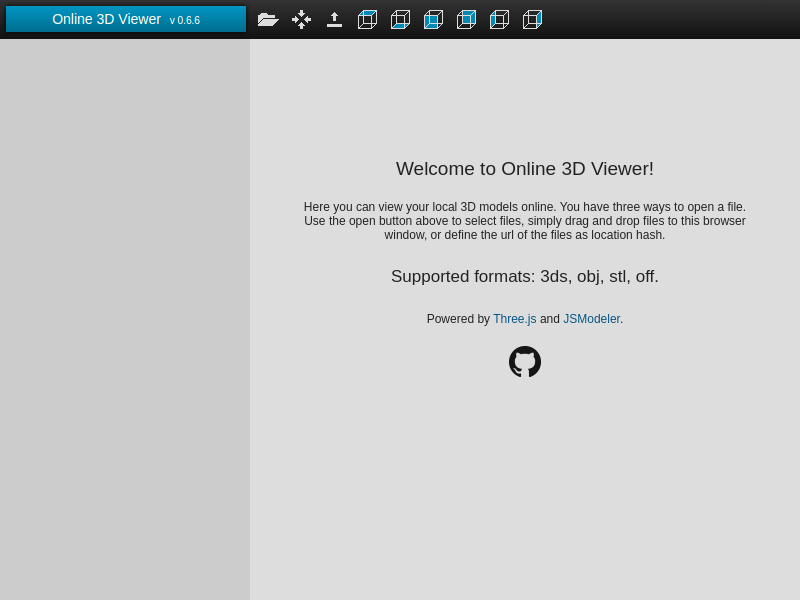
\includegraphics[width=\textwidth]{images/Model_Viewer.png}
\caption{Online 3D Viewer kezdőfelelület.}
\label{fig:model_viewer1}
\end{figure}

Mint \aref{fig:model_viewer1}. ábrán látható, a számunkra lényeges \texttt{.obj} kiterjesztésű fájl formátum szintén a támogatott fájlformátumok között szerepel.

A program leírásában benne van, hogy a megnyitás háromféleképpen történhet meg az oldal segitségével.
\begin{itemize}
\item Első lehetőségként az oldal bal felső részében található megnyitás gombra kattintva kiválasztjuk a megnyitni kivánt modellünket.
\item Második lehetőségként behúzzuk az oldalra a kívánt modellünket egér segítségével (\textit{drag-and-drop} művelet).
\item Harmadik lehetőség pedig megadhatjuk a fájlok helyének URL-jét.
\end{itemize}
\newpage
Miután kiválasztottuk a megfelelő objektumot az automatikusan megjelenik a rajzfelületen  (\ref{fig:model_viewer2}. ábra).

\begin{figure}[h]
\centering
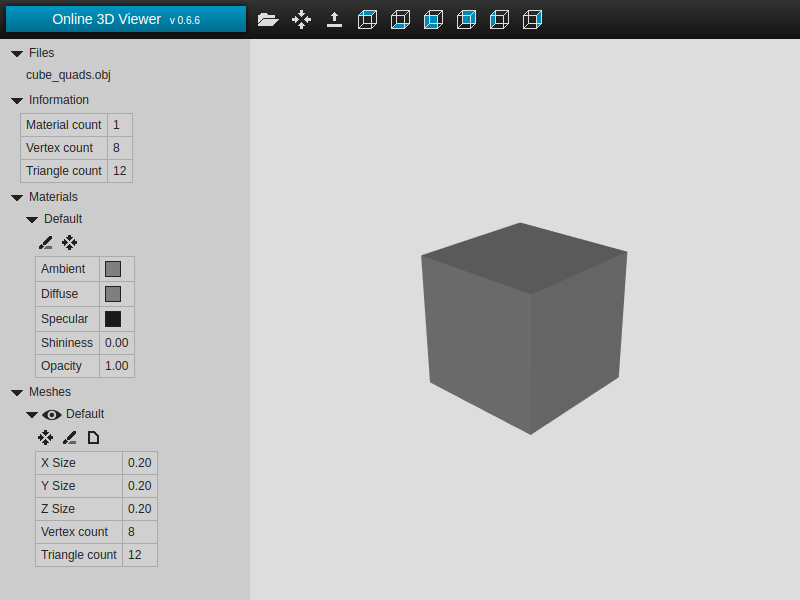
\includegraphics[width=\textwidth]{images/Model_Viewer_2.png}
\caption{Online 3D Viewer modell betöltéssel.}
\label{fig:model_viewer2}
\end{figure}

Rajzfelülettől balra találhatóak az objektumunkról gyűjtött adatok. Felette a model egyes síkidomjainak központba helyezése, a modellünk forgatása bal egérgomb folytonos nyomva tartásával és egér mozgatásával történhet. Ezen felül kameránk közelítése és távolítása görgő segítségével kivitelezhető.

A modellbetöltő gyors és egyszerű megjelenítést biztosít számunkra, tökéletesen működik a bonyolultabb geometriájú síkodomok megjelenítésével, legyen szó háromszög, négyszög vagy akár ennél nagyobb csúcsszámmal rendelkező sokszögről. Ez nagy előnyt jelent felhasználó szempontból, amennyiben csak a modell megjelenítése a cél.

Sajnos kép alapú textúrázás nem támogatott a program által, ezért a textúrázás nem lehetséges. Másik probléma a szoftverrel, hogy egy időben csak egy OBJ file kirajzolására alkalmas.

A betöltő forráskódja, illetve a programmal kapcsolatos rövid leírás megtalálható a következő weboldalon: \url{https://github.com/kovacsv/Online3DViewer}.
\newpage
\SubSection{Creators 3D Online Viewer}

Másik ilyen internetes betöltő a Creators 3D Online Viewer \cite{creators2018creators3d}.
Ennek weboldala a  \url{https://www.creators3d.com/online-viewer} címen található.

Hasonlóan az előző Online 3D Viewer-hez a betöltő kezdőfelületén \aref{fig:3d1}. ábra szintén tájékoztatást ad a támogatott fájlformátumokról.

Ez a betöltő is támogatja a OBJ fájl megjelenítését. A betöltő szintén támogatást nyújt a különböző számú csúcspontal rendelkező sokszögek betöltésével, az előzőtől eltérően itt a megnyitás kétféle képpen történhet.
\begin{itemize}
\item Első lehetőség:
A rajzfelültre húzzuk a megjelenítésre szánt objektum fájlunkat .
\item Második lehetőség:
Rajzfelületre kattintva megadjuk a fájlunk lokális helyének az útvonalát.
A rajzfelületre kattintva megadjuk a fájlunk lokális helyének az útvonalát.
\end{itemize}

\begin{figure}[h]
	\centering
	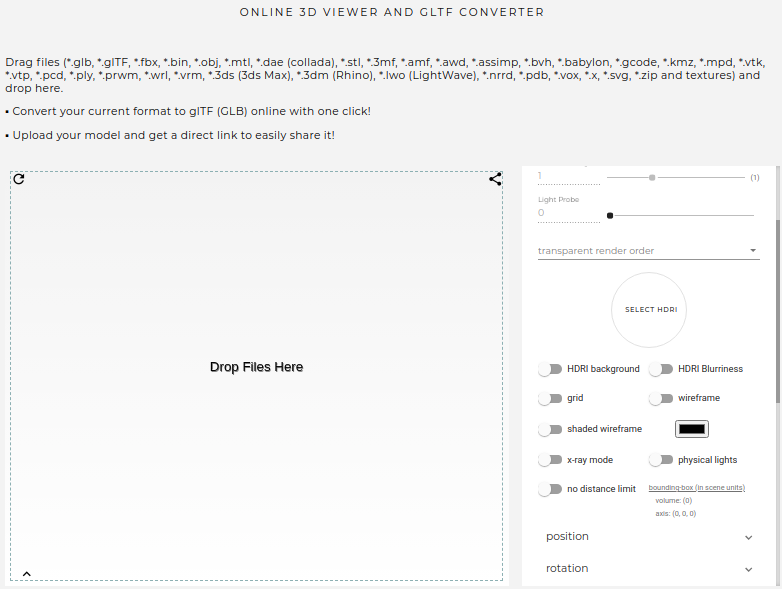
\includegraphics[width=\textwidth]{images/3D_creators.png}
	\caption{Online 3D Viewer kezdőfelület.}
	\label{fig:3d1}
\end{figure}
\newpage
Amint kiválasztjuk a megjelenítésre szánt fájlunkat a felsorolt két lehetőség közül, az objektum megjelenik a rajzfelületen (\ref{fig:3d2}. ábra).

\begin{figure}[h]
\centering
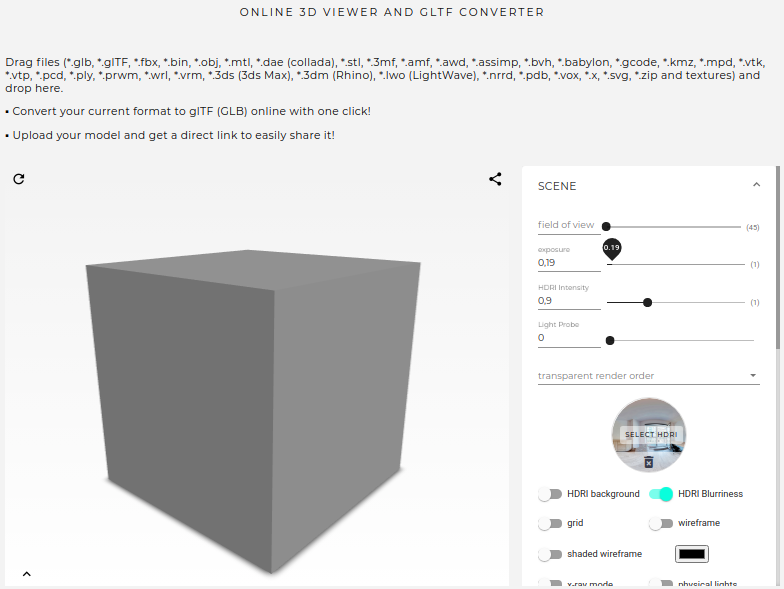
\includegraphics[width=\textwidth]{images/3D_creators_2.png}
\caption{Online 3D Viewer modell betöltéssel.}
\label{fig:3d2}
\end{figure}

Az előző betöltőhöz hasonlóan szintén nagyon gyorsan megjelenítette a betöltésre szánt modellünket. Nyilván minél komplexebb a modellünk, azzal arányosan több időbe telik a betöltés.
 \newpage
A rajzfelülettől jobbra találhatóak különböző beállítások a megjelenítéssel kapcsolatban. Ilyenek például a keret kirajzolása (\textit{wireframe}), aminek bekapcsolásával csak a modell hálója látszódik (\ref{fig:3d3}. ábra).

\begin{figure}[h]
\centering
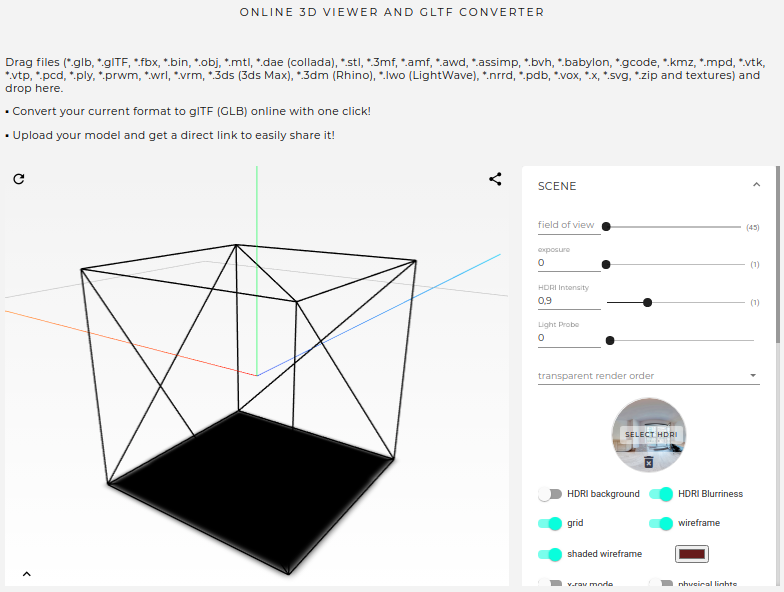
\includegraphics[width=\textwidth]{images/3D_creators_4.png}
\caption{Online 3D Viewer keret kirajzolással.}
\label{fig:3d3}
\end{figure}

Sok más további funkcióval is rendelkezik, például megjeleníthető a koordináta tengely (\textit{grid}), aminek segítségével vizsgálhatjuk az objektumunk irányultságát, illetve elhelyeszkedését. Az $x$, $y$ tengely kék és piros vonallal lettek jelezve a $z$ tengely pedig zöldel  (\ref{fig:3d3}. ábra).
\newpage
\SubSection{Model Loader}

Következő tesztelt szoftver, a Piller Imre által fejlesztett Model Loader volt \cite{imre2020model}.

A betöltő szoftverről részletes magyar nyelvű leírás és használati útmutató a következő webcímen található: \url{https://www.uni-miskolc.hu/~matip/grafika/}.

A weboldalon található teljes dokumentáció a következő részeket tartalmazza: fejlesztő környezet beüzemelése, egyszerű objektumok kirajzolás, anyagjellemzők beállítása, illetve textúrázás.

Ez a betöltő támogatja a kép alapú textúrázást, több objektum egy időben való betöltését. Ezeket akár különböző textúrával illetve anyagjellemzővel is megjeleníthetjük.

A fejlesztői környezet beállítása után az első futtatásra a \texttt{cube.obj} nevű példa a hozzátartozó textúrával \aref{fig:model1}. ábrán látható módon néz ki.

\begin{figure}[h]
\centering
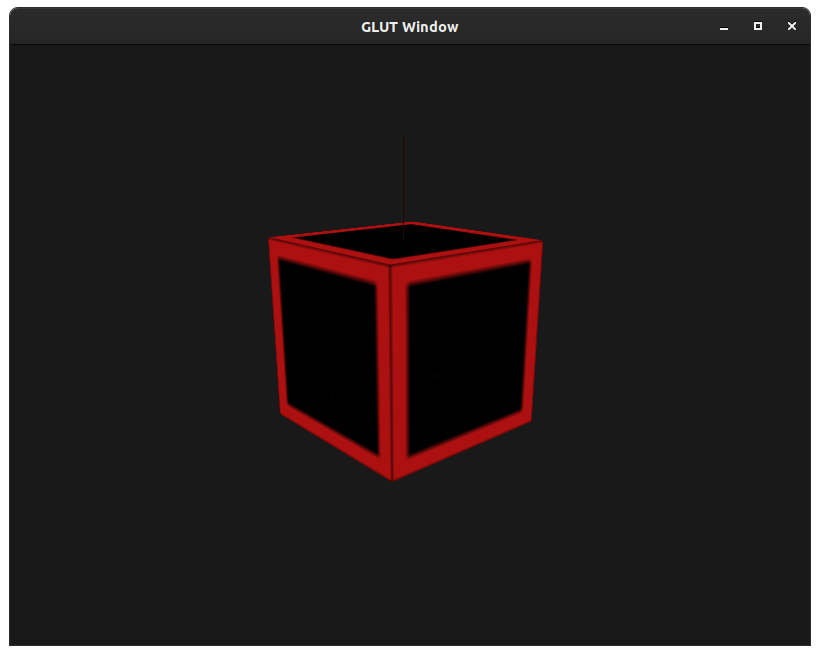
\includegraphics[width=\textwidth]{images/Model_loader.png}
\caption{Cube.obj megjelenítése.}
\label{fig:model1}
\end{figure}

A megjelenítés teljesen jól történ,t a megjelenítendő objektumot egy külön ablakban kirajzolta a program. A textúra illesztésével nem volt gond.
\newpage
Különböző komplexitású modellek betöltését teszteltem (\ref{fig:modelbaby}. és  \ref{fig:modelbird}. ábrák).

\begin{figure}[h]
\centering
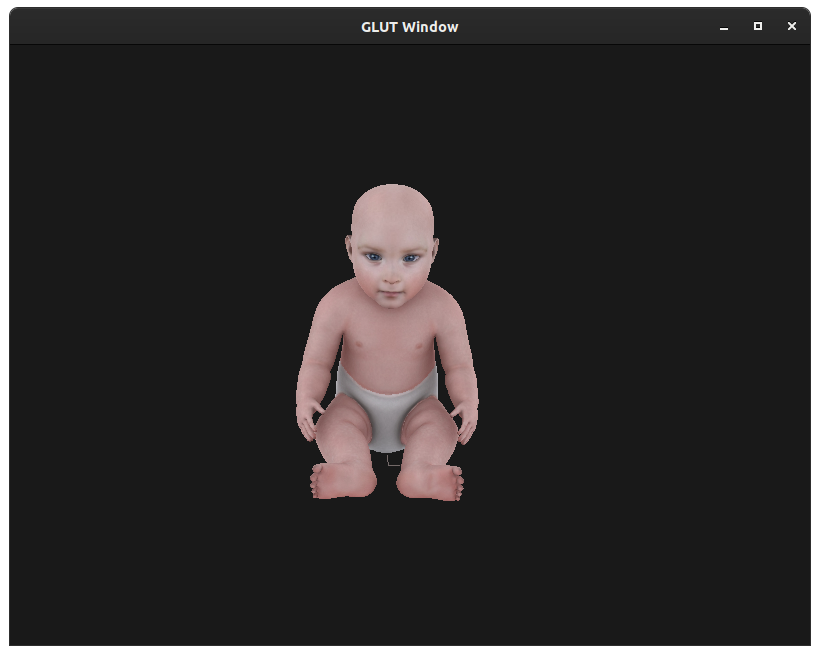
\includegraphics[scale=0.35]{images/model1.png}
\caption{Baby.obj modell megjelenítése.}
\label{fig:modelbaby}
\end{figure}

\begin{figure}[h]
\centering
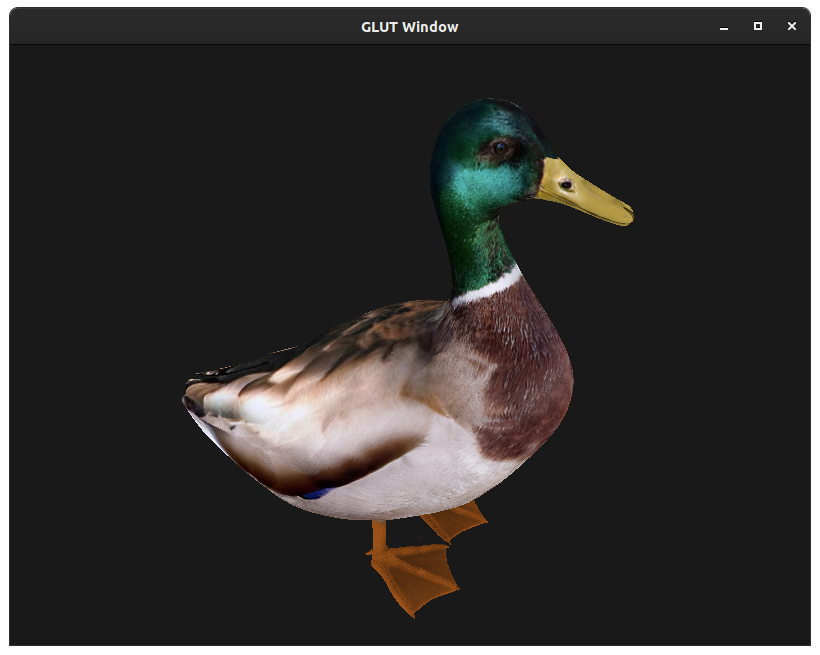
\includegraphics[scale=0.35]{images/bird.png}
\caption{Bird.obj modell megjelenítése.}
\label{fig:modelbird}
\end{figure}

Ezek a modellek szintén tökéletes megjelenítésre kerültek, a hozzájuk tartozó textúra betöltésével nem volt gond a modell megjelent a rajzfelületen.
\newpage
Pár ilyen betöltés után észrevettem, hogy a betöltő nem kezel háromszögnél nagyobb csúcspontal rendelkező sokszögeket. \Aref{fig:model1} ábrán megjelenített \texttt{cube.obj} háromszögeit átkonvertáltam négyszögekké, majd ezek után szintén betöltöttem a megjelenítőbe. A betöltés utáni eredmény \aref{fig:model2}. ábrán látható.

\begin{figure}[h]
\centering
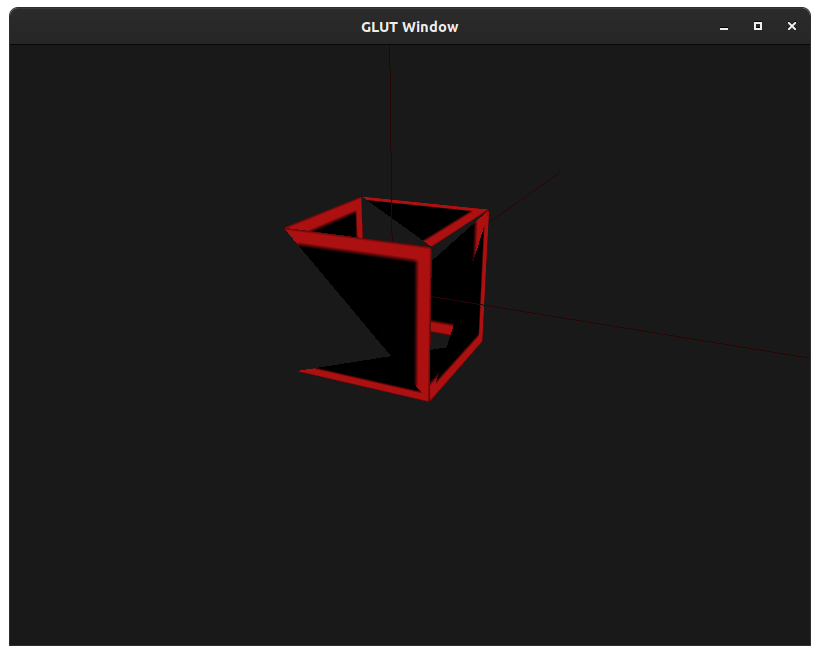
\includegraphics[width=\textwidth]{images/Model_quads.png}
\caption{Cube Model négyszögekkel.}
\label{fig:model2}
\end{figure}

Az ábrán jól látható, hogy az objektum megjelent az ablakban, viszont a kirajzolás nem megfelelő módon történt, a kockánk eléggé hiányos. Hiányzik a síkidomokról a negyedik csúcspont. A javító programunk egyik tervezett része ennek a hibának a javítására szolgál.
